\documentclass[aspectratio=169]{beamer}

\usetheme{Madrid}
\usecolortheme{dolphin}
\setbeamertemplate{navigation symbols}{}
\setbeamertemplate{footline}[frame number]

\usepackage{amsmath,amssymb}
\usepackage{graphicx}
\usepackage{booktabs}
\usepackage{tikz}
\usetikzlibrary{arrows.meta, positioning, shapes}
\usepackage{pgfplots}
\pgfplotsset{compat=1.17}

% Speaker notes
\usepackage{pgfpages}
% Uncomment one of these depending on how you want notes
%\setbeameroption{show notes} % show notes under slides
%\setbeameroption{show notes on second screen=right}

% Custom colors for highlighting
\definecolor{keyblue}{RGB}{0,102,204}
\definecolor{statecolor}{RGB}{255,200,150}
\definecolor{actioncolor}{RGB}{180,210,255}
\definecolor{rewardcolor}{RGB}{255,255,180}
\setbeamercolor{block title}{bg=keyblue,fg=white}
\setbeamercolor{block body}{bg=keyblue!10}

% Checkmark for roadmap
\usepackage{pifont}
\newcommand{\cmark}{\ding{51}}

% Placeholder for missing figures
\newcommand{\figurePlaceholder}[1]{%
  \begin{tikzpicture}
    \draw[dashed, gray, thick] (0,0) rectangle (4,2.5);
    \node[text width=3.5cm, align=center, font=\small\itshape] at (2,1.25) {#1};
  \end{tikzpicture}%
}

%============================================================================
% SPEAKER ASSIGNMENTS (25 min total + 5 min QA)
%============================================================================
% Speaker 1 (Pegah):  Background & Motivation       - Slides 1-9   (~5 min)
% Speaker 2 (Danielle):    Problem Formulation & Fenchel - Slides 10-17 (~5 min)
% Speaker 3 (Shervin):    Related Work & Our Method     - Slides 18-26 (~6 min)
% Speaker 4 (Ahmed): Experiments & Conclusion      - Slides 27-35 (~6 min)
%============================================================================

\title{A Dual--SPMA Framework for Convex MDPs}
\subtitle{Fenchel Duality + Softmax Policy Mirror Ascent}
\author{Shervin Khamooshian \and Ahmed Magd \and Pegah Aryadoost \and Danielle Nguyen}
\institute{School of Computing Science, Simon Fraser University}
\date{Project Presentation}

\begin{document}

%============================================================================
% SLIDE 1: Title
%============================================================================
\begin{frame}
  \titlepage
  \vspace{-0.5em}
  \begin{block}{Main Claim}
  Fenchel duality + a fast policy optimizer (SPMA) gives a simple, competitive way to solve convex MDPs; we compare this Dual--SPMA recipe against NPG--PD.
  \end{block}
  
  \note{
    \textbf{Slide 1 --- Speaker 1 (Shervin) starts}
    \begin{itemize}
      \item Welcome and introduce the project title.
      \item Read the one-sentence claim in the box.
      \item Briefly mention group members and that each will handle different sections.
    \end{itemize}
  }
\end{frame}

%============================================================================
% SLIDE 2: Outline
%============================================================================
\begin{frame}{Outline}
  % Manual outline (more reliable than \tableofcontents which needs 2 compilations)
  \begin{enumerate}
    \item \textcolor{keyblue}{Background: Reinforcement Learning}
    \item \textcolor{keyblue}{Motivation: Convex MDPs}
    \item \textcolor{keyblue}{Problem Formulation: Fenchel Duality}
    \item \textcolor{keyblue}{Related Work: ``Reward Is Enough'' \& SPMA}
    \item \textcolor{keyblue}{Our Method: Dual--SPMA}
    \item \textcolor{keyblue}{Experiments}
    \item \textcolor{keyblue}{Conclusion \& Future Work}
  \end{enumerate}
  \note{
    \textbf{Slide 2}
    \begin{itemize}
      \item Walk through the outline quickly (30 seconds max).
      \item Background covers RL basics for the class.
      \item Then convex MDPs, Fenchel duality, related work.
      \item Finally our method, experiments, and conclusions.
    \end{itemize}
  }
\end{frame}

%============================================================================
\section{Background: Reinforcement Learning}
%============================================================================

%============================================================================
% SLIDE 3: What is RL?
%============================================================================
\begin{frame}{What is Reinforcement Learning?}
  \textbf{Reinforcement Learning (RL)} is a learning framework where an agent learns to make decisions by interacting with an environment.
  
  \vspace{0.5cm}
  \begin{columns}
    \column{0.55\textwidth}
    At each time step $t$, the agent:
    \begin{enumerate}
      \item Observes a \textbf{state} $s_t$
      \item Chooses an \textbf{action} $a_t$ (based on a policy)
      \item Receives a \textbf{reward} $r_t$
      \item Transitions to a new \textbf{state} $s_{t+1}$
    \end{enumerate}
    
    \column{0.42\textwidth}
    \begin{center}
      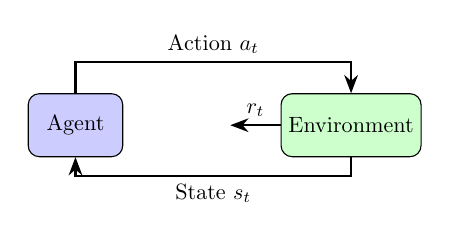
\begin{tikzpicture}[node distance=1.2cm, >=Stealth, scale=0.8, transform shape]
        % Agent
        \node[draw, rounded corners, fill=blue!20, minimum width=1.5cm, minimum height=1cm] (agent) {Agent};
        % Environment
        \node[draw, rounded corners, fill=green!20, minimum width=1.5cm, minimum height=1cm, right=2.5cm of agent] (env) {Environment};
        
        % Arrows
        \draw[->, thick] (agent.north) -- ++(0,0.5) -| node[pos=0.25, above] {Action $a_t$} (env.north);
        \draw[->, thick] (env.south) -- ++(0,-0.3) -| node[pos=0.25, below] {State $s_t$} (agent.south);
        \draw[->, thick] (env.west) -- ++(-0.8,0) node[midway, above] {$r_t$};
      \end{tikzpicture}
    \end{center}
  \end{columns}

  \note{
    \textbf{Slide 3}
    \begin{itemize}
      \item This is background for the class---many may not know RL.
      \item Explain the agent-environment loop intuitively.
      \item The goal is to learn a good policy through trial and error.
    \end{itemize}
  }
\end{frame}

%============================================================================
% SLIDE 4: MDP Definition
%============================================================================
\begin{frame}{Markov Decision Process (MDP): Formal Definition}
  An \textbf{MDP} is defined by the tuple $(\mathcal{S}, \mathcal{A}, P, r, \gamma, \rho)$:
  
  \vspace{0.3cm}
  \begin{center}
  \begin{tabular}{cl}
    \toprule
    \textbf{Symbol} & \textbf{Meaning} \\
    \midrule
    $\mathcal{S}$ & State space (set of all possible states) \\
    $\mathcal{A}$ & Action space (set of all possible actions) \\
    $P(s'|s,a)$ & Transition probability: probability of reaching $s'$ from $(s,a)$ \\
    $r(s,a)$ & Reward function: immediate reward for taking action $a$ in state $s$ \\
    $\gamma \in [0,1)$ & Discount factor: how much to value future vs.\ immediate rewards \\
    $\rho(s)$ & Initial state distribution \\
    \bottomrule
  \end{tabular}
  \end{center}
  
  \vspace{0.3cm}
  \textbf{Policy} $\pi(a|s)$: probability of taking action $a$ in state $s$.

  \note{
    \textbf{Slide 4}
    \begin{itemize}
      \item Define all the notation carefully---professor wants this.
      \item Emphasize that $\gamma$ controls short-term vs long-term thinking.
      \item Policy can be deterministic or stochastic.
    \end{itemize}
  }
\end{frame}

%============================================================================
% SLIDE 5: Trajectory and Return
%============================================================================
\begin{frame}{Trajectory and Return}
  A \textbf{trajectory} $\tau$ is a sequence of states, actions, and rewards:
  
  \vspace{0.1cm}
  \begin{center}
  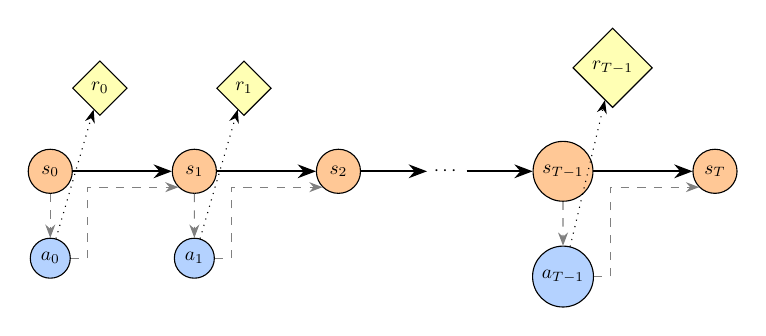
\begin{tikzpicture}[>=Stealth, scale=0.7, transform shape]
    % States
    \node[draw, circle, fill=statecolor, minimum size=0.8cm] (s0) {$s_0$};
    \node[draw, circle, fill=statecolor, minimum size=0.8cm, right=1.8cm of s0] (s1) {$s_1$};
    \node[draw, circle, fill=statecolor, minimum size=0.8cm, right=1.8cm of s1] (s2) {$s_2$};
    \node[right=1.2cm of s2] (dots) {$\cdots$};
    \node[draw, circle, fill=statecolor, minimum size=0.8cm, right=1.2cm of dots] (sT1) {$s_{T-1}$};
    \node[draw, circle, fill=statecolor, minimum size=0.8cm, right=1.8cm of sT1] (sT) {$s_T$};
    
    % Actions
    \node[draw, circle, fill=actioncolor, minimum size=0.6cm, below=0.8cm of s0] (a0) {$a_0$};
    \node[draw, circle, fill=actioncolor, minimum size=0.6cm, below=0.8cm of s1] (a1) {$a_1$};
    \node[draw, circle, fill=actioncolor, minimum size=0.6cm, below=0.8cm of sT1] (aT1) {$a_{T-1}$};
    
    % Rewards
    \node[draw, diamond, fill=rewardcolor, minimum size=0.5cm, above=0.6cm of s0, xshift=0.9cm] (r0) {$r_0$};
    \node[draw, diamond, fill=rewardcolor, minimum size=0.5cm, above=0.6cm of s1, xshift=0.9cm] (r1) {$r_1$};
    \node[draw, diamond, fill=rewardcolor, minimum size=0.5cm, above=0.6cm of sT1, xshift=0.9cm] (rT1) {$r_{T-1}$};
    
    % State transitions
    \draw[->, thick] (s0) -- (s1);
    \draw[->, thick] (s1) -- (s2);
    \draw[->, thick] (s2) -- (dots);
    \draw[->, thick] (dots) -- (sT1);
    \draw[->, thick] (sT1) -- (sT);
    
    % Action arrows
    \draw[->, dashed, gray] (s0) -- (a0);
    \draw[->, dashed, gray] (a0.east) -- ++(0.3,0) |- (s1.south west);
    \draw[->, dashed, gray] (s1) -- (a1);
    \draw[->, dashed, gray] (a1.east) -- ++(0.3,0) |- (s2.south west);
    \draw[->, dashed, gray] (sT1) -- (aT1);
    \draw[->, dashed, gray] (aT1.east) -- ++(0.3,0) |- (sT.south west);
    
    % Reward arrows
    \draw[->, dotted] (a0) -- (r0);
    \draw[->, dotted] (a1) -- (r1);
    \draw[->, dotted] (aT1) -- (rT1);
  \end{tikzpicture}
  \end{center}
  
  \vspace{0.1cm}
  \begin{block}{Discounted Return}
  \small The \textbf{expected discounted return} under policy $\pi$ is:
  $J(\pi) = \mathbb{E}_\pi\left[ \sum_{t=0}^{\infty} \gamma^t r(s_t, a_t) \right]$
  \end{block}
  
  \vspace{-0.1cm}
  \textbf{Goal of RL:} Find $\pi^\star = \arg\max_\pi J(\pi)$

  \note{
    \textbf{Slide 5}
    \begin{itemize}
      \item The trajectory diagram shows the sequential nature of RL.
      \item Rewards are discounted by $\gamma^t$---future rewards worth less.
      \item Goal is to find the policy that maximizes expected return.
    \end{itemize}
  }
\end{frame}

%============================================================================
% SLIDE 6: Occupancy measure
%============================================================================
\begin{frame}{Occupancy Measure: Where the Policy Spends Time}
  \begin{columns}
    \column{0.55\textwidth}
    \begin{block}{Discounted Occupancy Measure}
    \[
    d_\pi(s,a) = (1-\gamma)\sum_{t=0}^\infty \gamma^t \Pr_\pi(s_t=s,a_t=a)
    \]
    \end{block}
    
    \textbf{Notation:}
    \begin{itemize}
      \item $d_\pi(s,a)$: probability of being in state $s$ and taking action $a$ under policy $\pi$
      \item $(1-\gamma)$: normalization factor
      \item $\Pr_\pi$: probability under policy $\pi$
    \end{itemize}
    
    \column{0.42\textwidth}
    \begin{center}
      % Placeholder heatmap visualization
      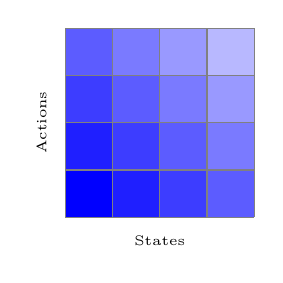
\begin{tikzpicture}[scale=0.6]
        \foreach \x in {0,1,2,3} {
          \foreach \y in {0,1,2,3} {
            \pgfmathsetmacro{\intensity}{100-(\x+\y)*12}
            \fill[blue!\intensity] (\x,\y) rectangle (\x+1,\y+1);
          }
        }
        \draw[step=1,gray,thin] (0,0) grid (4,4);
        \node at (2,-0.5) {\tiny States};
        \node[rotate=90] at (-0.5,2) {\tiny Actions};
      \end{tikzpicture}
      
      {\small Think of $d_\pi$ as a \textbf{heatmap}: bright = often visited}
    \end{center}
  \end{columns}
  
  \vspace{0.2cm}
  \textbf{Key property:} $d_\pi$ is a probability distribution: $\sum_{s,a} d_\pi(s,a) = 1$

  \note{
    \textbf{Slide 6}
    \begin{itemize}
      \item Define $d_\pi$ formally and explain each symbol.
      \item Use the heatmap figure to give intuition.
      \item Point out that $\sum_{s,a} d_\pi(s,a) = 1$.
    \end{itemize}
  }
\end{frame}

%============================================================================
% SLIDE 7: RL is linear in occupancy
%============================================================================
\begin{frame}{Key Identity: RL is Linear in Occupancy}
  \begin{block}{Fundamental Identity}
  \vspace{-0.2cm}
  \[
  \langle r, d_\pi \rangle = \sum_{s,a} r(s,a)\, d_\pi(s,a) = (1-\gamma)\, J(\pi)
  \]
  \vspace{-0.2cm}
  \end{block}
  
  \textbf{What does this mean?}
  \begin{itemize}\setlength{\itemsep}{0pt}
    \item Up to the constant $(1-\gamma)$, the RL objective is \textbf{linear} in $d_\pi$
    \item Weights = how often we visit each $(s,a)$ pair
    \item Standard RL $\Rightarrow$ maximize a \textbf{linear} function of $d_\pi$
  \end{itemize}
  
  \vspace{0.1cm}
  \textbf{But many interesting goals are NOT linear in $d_\pi$:}
  \begin{center}
  \small
  \begin{tabular}{ll}
    \toprule
    \textbf{Goal} & \textbf{Objective} \\
    \midrule
    Safety constraints & $\max J_r(\pi)$ subject to $\langle c, d_\pi \rangle \le \tau$ \\
    Imitation learning & $\min \|d_\pi - d_{\text{expert}}\|$ \\
    Exploration & $\max J_r(\pi) + \alpha H(d_\pi)$ \\
    \bottomrule
  \end{tabular}
  \end{center}

  \note{
    \textbf{Slide 7}
    \begin{itemize}
      \item This identity is the bridge to convex MDPs.
      \item Emphasize that standard RL is linear in occupancy.
      \item But constraints, imitation, exploration need more general objectives.
    \end{itemize}
  }
\end{frame}

%============================================================================
\section{Motivation: Convex MDPs}
%============================================================================

%============================================================================
% SLIDE 8: Why Convex MDPs
%============================================================================
\begin{frame}{Why Convex MDPs?}
  \begin{columns}
    \column{0.48\textwidth}
    \textbf{Problem:} Linear RL is insufficient for:
    \begin{itemize}
      \item Safety constraints
      \item Matching expert behavior
      \item Encouraging exploration
      \item Risk-sensitive objectives
    \end{itemize}
    
    \vspace{0.3cm}
    \textbf{Solution:} Convex MDPs
    \[
    \min_{\pi} f(d_\pi)
    \]
    where $f$ is a \textbf{convex function}
    
    \column{0.48\textwidth}
    \textbf{Challenge:}
    \begin{itemize}
      \item Optimizing over occupancy measures is hard
      \item High-dimensional constrained space
      \item Can't directly apply standard RL
    \end{itemize}
    
    \vspace{0.3cm}
    \textbf{Our approach:}
    \begin{itemize}
      \item Use \textbf{Fenchel duality}
      \item Transform to min-max game
      \item Reduce to shaped-reward RL
    \end{itemize}
  \end{columns}

  \note{
    \textbf{Slide 8}
    \begin{itemize}
      \item Motivate why we need convex MDPs.
      \item The challenge is that direct optimization is hard.
      \item Preview our solution: Fenchel duality.
    \end{itemize}
  }
\end{frame}

%============================================================================
% SLIDE 9: Convex MDP Examples
%============================================================================
\begin{frame}{Convex MDP: Examples}
  \begin{block}{General Form}
  $\min_{d \in \mathcal{D}} f(d)$ where $\mathcal{D}$ = feasible occupancy measures, $f$ = convex
  \end{block}
  
  \vspace{0.3cm}
  \textbf{Example 1: Standard RL} (linear, trivially convex)
  \[
  f(d) = -\langle r, d \rangle = -\sum_{s,a} r(s,a)\, d(s,a)
  \]
  
  \textbf{Example 2: Entropy-Regularized RL}
  \[
  f(d) = -\langle r, d \rangle + \alpha \sum_{s,a} d(s,a) \log d(s,a)
  \]
  
  \textbf{Example 3: Constrained Safety (CMDP)}
  \[
  f(d) = -\langle r, d \rangle + \mu \max\{0, \langle c, d \rangle - \tau\}
  \]
  where $c(s,a)$ = cost function, $\tau$ = threshold, $\mu$ = fixed penalty weight

  \note{
    \textbf{Slide 9 --- End of Speaker 1's section}
    \begin{itemize}
      \item Show concrete examples of convex objectives.
      \item Standard RL is a special case (linear).
      \item Entropy and safety constraints are truly convex.
      \item Note: $\mu$ here is a fixed penalty weight, not the CMDP dual variable $\lambda$ used later.
      \item Transition to Speaker 2 for Fenchel duality.
    \end{itemize}
  }
\end{frame}

%============================================================================
\section{Problem Formulation: Fenchel Duality}
%============================================================================

%============================================================================
% SLIDE 10: Roadmap
%============================================================================
\begin{frame}{Roadmap}
  \begin{enumerate}
    \item[\cmark] Background: Reinforcement Learning
    \item[\cmark] Motivation: Convex MDPs
    \item[$\rightarrow$] \textbf{Problem Formulation: Fenchel Duality}
    \item[] Related Work: ``Reward Is Enough'' \& SPMA
    \item[] Our Method: Dual--SPMA
    \item[] Experiments
    \item[] Conclusion \& Future Work
  \end{enumerate}
  
  \note{
    \textbf{Slide 10 --- Speaker 2 (Ahmed) starts}
    \begin{itemize}
      \item Quick roadmap reminder.
      \item Now we'll derive the Fenchel dual step by step.
    \end{itemize}
  }
\end{frame}

%============================================================================
% SLIDE 11: Fenchel Conjugate Definition
%============================================================================
\begin{frame}{Fenchel Conjugate: Definition}
  Given a convex function $f: \mathbb{R}^n \to \mathbb{R} \cup \{\infty\}$
  
  \begin{block}{Fenchel Conjugate (Convex Conjugate)}
  \[
  f^\ast(y) = \sup_{x \in \mathbb{R}^n} \left\{ \langle y, x \rangle - f(x) \right\}
  \]
  \end{block}
  
  \textbf{Notation:}
  \begin{itemize}
    \item $f^\ast(y)$: the conjugate function evaluated at dual variable $y$
    \item $\langle y, x \rangle = \sum_i y_i x_i$: inner product (dot product)
    \item $\sup$: supremum (least upper bound)
  \end{itemize}
  
  \vspace{0.2cm}
  \textbf{Intuition:} $f^\ast(y)$ measures ``how much $\langle y, x \rangle$ can exceed $f(x)$''
  
  % Figure removed - geometric intuition explained verbally

  \note{
    \textbf{Slide 11}
    \begin{itemize}
      \item Define the Fenchel conjugate carefully.
      \item Explain each symbol.
      \item Give geometric intuition if time permits.
    \end{itemize}
  }
\end{frame}

%============================================================================
% SLIDE 12: Fenchel-Moreau Identity
%============================================================================
\begin{frame}{Fenchel--Moreau Theorem}
  \begin{block}{Fenchel--Moreau Identity}
  For any proper, closed, convex function $f$:
  \[
  f(d) = \sup_{y} \left\{ \langle y, d \rangle - f^\ast(y) \right\}
  \]
  \end{block}
  
  \textbf{What does this say?}
  \begin{itemize}
    \item We can \textbf{recover} $f$ from its conjugate $f^\ast$
    \item $f$ is the conjugate of its conjugate: $f = (f^\ast)^\ast$
    \item This is called \textbf{biconjugation}
  \end{itemize}
  
  \vspace{0.3cm}
  \textbf{Why is this useful?}
  \begin{itemize}
    \item Transforms a minimization problem into a \textbf{min-max} problem
    \item Introduces a \textbf{dual variable} $y$ that we can optimize over
  \end{itemize}

  \note{
    \textbf{Slide 12}
    \begin{itemize}
      \item State the Fenchel-Moreau theorem.
      \item Emphasize that this lets us recover $f$ from $f^\ast$.
      \item Key insight: transforms min to min-max.
    \end{itemize}
  }
\end{frame}

%============================================================================
% SLIDE 13: Applying to Convex MDP
%============================================================================
\begin{frame}{Applying Fenchel Duality to Convex MDPs}
  \textbf{Step 1:} Start with the convex MDP problem
  \[
  \min_{d \in \mathcal{D}} f(d)
  \]
  
  \textbf{Step 2:} Apply Fenchel--Moreau identity
  \[
  \min_{d \in \mathcal{D}} f(d) = \min_{d \in \mathcal{D}} \sup_{y} \left\{ \langle y, d \rangle - f^\ast(y) \right\}
  \]
  
  \textbf{Step 3:} This is a \textbf{convex-concave saddle-point problem}
  \[
  = \min_{d \in \mathcal{D}} \max_{y} \left\{ \langle y, d \rangle - f^\ast(y) \right\}
  \]
  {\small (Under standard conditions, solving this saddle-point is equivalent to the original problem.)}
  
  \textbf{Step 4:} Replace $d$ with $d_\pi$ (occupancy induced by policy)
  \begin{block}{Saddle-Point Formulation}
  \vspace{-0.2cm}
  \[
  \min_{\pi} \max_{y} \underbrace{\langle y, d_\pi \rangle - f^\ast(y)}_{L(\pi, y)}
  \]
  \vspace{-0.3cm}
  \end{block}

  \note{
    \textbf{Slide 13}
    \begin{itemize}
      \item Walk through the derivation step by step.
      \item Avoid saying ``swap min/max''---we just recognize it as a saddle-point problem.
      \item End with the saddle-point formulation.
    \end{itemize}
  }
\end{frame}

%============================================================================
% SLIDE 14: Two-Player Game Interpretation
%============================================================================
\begin{frame}{Two-Player Game Interpretation}
  \begin{block}{Saddle-Point Problem}
  \[
  \min_{\pi} \max_{y} L(\pi, y), \quad \text{where } L(\pi, y) = \langle y, d_\pi \rangle - f^\ast(y)
  \]
  \end{block}
  
  This is a \textbf{min-max game} between two players:
  
  \vspace{0.3cm}
  \begin{columns}
    \column{0.48\textwidth}
    \begin{center}
    \textbf{Policy Player (min)}
    \end{center}
    \begin{itemize}
      \item Chooses policy $\pi$
      \item Wants to minimize $L$
      \item Controls occupancy $d_\pi$
    \end{itemize}
    
    \column{0.48\textwidth}
    \begin{center}
    \textbf{Dual Player (max)}
    \end{center}
    \begin{itemize}
      \item Chooses dual variable $y$
      \item Wants to maximize $L$
      \item Shapes the reward signal
    \end{itemize}
  \end{columns}
  
  \vspace{0.5cm}
  \begin{center}
  \fbox{\parbox{0.8\textwidth}{\centering
    At equilibrium: policy player finds optimal $\pi^\ast$,\\
    dual player finds optimal $y^\ast$
  }}
  \end{center}

  \note{
    \textbf{Slide 14}
    \begin{itemize}
      \item Interpret the saddle-point as a two-player game.
      \item Policy player minimizes, dual player maximizes.
      \item This game-theoretic view motivates alternating updates.
    \end{itemize}
  }
\end{frame}

%============================================================================
% SLIDE 15: Saddle Point Visualization
%============================================================================
\begin{frame}{Visualizing the Saddle Point}
  \begin{columns}
    \column{0.55\textwidth}
    \begin{center}
    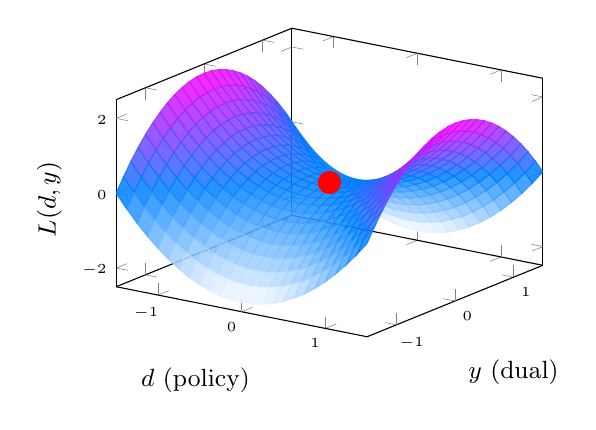
\begin{tikzpicture}
      \begin{axis}[
        width=7cm,
        height=5.5cm,
        view={35}{25},
        xlabel={$d$ (policy)},
        ylabel={$y$ (dual)},
        zlabel={$L(d,y)$},
        xlabel style={font=\small},
        ylabel style={font=\small},
        zlabel style={font=\small},
        tick label style={font=\tiny},
        colormap/cool,
        samples=25,
        domain=-1.5:1.5,
        y domain=-1.5:1.5,
        zmin=-2.5, zmax=2.5,
      ]
        % Saddle surface: z = x^2 - y^2
        \addplot3[surf, opacity=0.85, shader=flat] {x^2 - y^2};
        
        % Red dot at saddle point
        \addplot3[only marks, mark=*, mark size=4pt, color=red] 
          coordinates {(0, 0, 0)};
      \end{axis}
    \end{tikzpicture}
    \end{center}
    
    \column{0.45\textwidth}
    \textbf{Min-max solution:}
    \[
    \min_d \max_y L(d,y)
    \]
    
    \vspace{0.2cm}
    At the \textcolor{red}{\textbf{red point}} (saddle point):
    \begin{itemize}
      \item Along $d$-direction: \textbf{minimal}
      \item Along $y$-direction: \textbf{maximal}
    \end{itemize}
    
    \vspace{0.2cm}
    \fbox{\parbox{0.9\linewidth}{\small\centering
      Policy player (min) and dual player (max) reach \textbf{equilibrium} here.
    }}
  \end{columns}

  \note{
    \textbf{Slide 15 --- Saddle Point Visualization}
    \begin{itemize}
      \item Point to the red dot: this is where both players are satisfied.
      \item Along the policy direction, we're at a minimum.
      \item Along the dual direction, we're at a maximum.
      \item This is the solution we're looking for!
    \end{itemize}
  }
\end{frame}

%============================================================================
% SLIDE 16: From Saddle Point to Shaped Reward
%============================================================================
\begin{frame}{From Saddle Point to Shaped Reward}
  \small
  For \textbf{fixed} dual variable $y$, the policy player solves:
  $\displaystyle\min_{\pi} \langle y, d_\pi \rangle$
  
  \vspace{0.2cm}
  Expand using the occupancy definition:
  \[
  \langle y, d_\pi \rangle = \sum_{s,a} y(s,a) \cdot d_\pi(s,a) = (1-\gamma) \mathbb{E}_\pi\left[ \sum_{t=0}^{\infty} \gamma^t y(s_t, a_t) \right]
  \]
  
  \vspace{-0.2cm}
  \begin{block}{Key Insight: Shaped Reward}
  \vspace{-0.1cm}
  \[
  \min_\pi \langle y, d_\pi \rangle = \min_\pi \mathbb{E}_\pi\left[ \sum_{t=0}^{\infty} \gamma^t y(s_t, a_t) \right] = \max_\pi \mathbb{E}_\pi\left[ \sum_{t=0}^{\infty} \gamma^t \underbrace{(-y(s_t, a_t))}_{r_y(s_t, a_t)} \right]
  \]
  \vspace{-0.2cm}
  \end{block}
  
  \textbf{Conclusion:} Policy player just does \textbf{standard RL} with shaped reward:
  $\boxed{r_y(s,a) = -y(s,a)}$

  \note{
    \textbf{Slide 15}
    \begin{itemize}
      \item Show how the policy step becomes shaped-reward RL.
      \item The key is that $\langle y, d_\pi \rangle$ is a discounted return.
      \item This means we can use ANY RL algorithm as the policy player!
    \end{itemize}
  }
\end{frame}

%============================================================================
% SLIDE 16: Summary of Reduction
%============================================================================
\begin{frame}{Summary: The Fenchel Dual Reduction}
  \begin{center}
  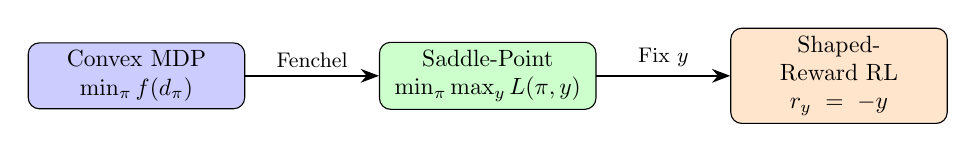
\begin{tikzpicture}[node distance=1.5cm, >=Stealth, scale=0.85, transform shape]
    \node[draw, rounded corners, fill=blue!20, text width=3cm, align=center] (cvx) {Convex MDP\\$\min_\pi f(d_\pi)$};
    \node[draw, rounded corners, fill=green!20, text width=3cm, align=center, right=2cm of cvx] (saddle) {Saddle-Point\\$\min_\pi \max_y L(\pi,y)$};
    \node[draw, rounded corners, fill=orange!20, text width=3cm, align=center, right=2cm of saddle] (rl) {Shaped-Reward RL\\$r_y = -y$};
    
    \draw[->, thick] (cvx) -- node[above] {\small Fenchel} (saddle);
    \draw[->, thick] (saddle) -- node[above] {\small Fix $y$} (rl);
  \end{tikzpicture}
  \end{center}
  
  \vspace{0.5cm}
  \textbf{Algorithm structure:}
  \begin{enumerate}
    \item \textbf{Dual step:} Update $y$ using gradient of $L$ w.r.t.\ $y$
    \[
    y_{k+1} = y_k + \alpha \left( d_{\pi_k} - \nabla f^\ast(y_k) \right)
    \]
    \item \textbf{Policy step:} Run RL algorithm with reward $r_{y_k} = -y_k$
    \[
    \pi_{k+1} = \text{RL-Update}(\pi_k, r_{y_k})
    \]
  \end{enumerate}

  \note{
    \textbf{Slide 16}
    \begin{itemize}
      \item Summarize the entire reduction in one slide.
      \item Show the pipeline: convex MDP $\to$ saddle $\to$ shaped RL.
      \item Give the alternating update structure.
    \end{itemize}
  }
\end{frame}

%============================================================================
% SLIDE 17: Roadmap (Transition to Related Work)
%============================================================================
\begin{frame}{Roadmap}
  \begin{enumerate}
    \item[\cmark] Background: Reinforcement Learning
    \item[\cmark] Motivation: Convex MDPs
    \item[\cmark] Problem Formulation: Fenchel Duality
    \item[$\rightarrow$] \textbf{Related Work: ``Reward Is Enough'' \& SPMA}
    \item[] Our Method: Dual--SPMA
    \item[] Experiments
    \item[] Conclusion \& Future Work
  \end{enumerate}
  
  \vspace{0.5cm}
  \begin{block}{Where We Are}
  We've established the Fenchel dual reduction. Now we review the key papers that inform our method: the theoretical foundation and the policy optimizer we'll use.
  \end{block}

  \note{
    \textbf{Slide 17 --- Roadmap / Speaker 3 (Pegah) starts}
    \begin{itemize}
      \item Quick checkpoint: we've covered the math behind the reduction.
      \item Now we'll look at the papers that make this practical.
      \item Zahavy et al.\ gives the theory, SPMA gives the fast policy learner.
    \end{itemize}
  }
\end{frame}

%============================================================================
\section{Related Work}
%============================================================================

%============================================================================
% SLIDE 18: Reward Is Enough Paper
%============================================================================
\begin{frame}{Related Work: ``Reward Is Enough'' (Zahavy et al., 2021)}
  \textbf{Main contributions of this foundational paper:}
  
  \begin{enumerate}
    \item \textbf{Fenchel dual reduction:}
      \begin{itemize}
        \item Reformulate convex MDP as saddle-point problem
        \item The theoretical foundation we just presented
      \end{itemize}
    
    \item \textbf{Meta-algorithm:}
      \begin{itemize}
        \item Alternating updates between policy and dual players
        \item Any RL algorithm can be the policy player
        \item Any online convex optimization (OCO) can be the dual player
      \end{itemize}
    
    \item \textbf{Unification:}
      \begin{itemize}
        \item Shows many RL paradigms are special cases of convex MDPs
        \item Imitation learning, constrained RL, entropy-regularized RL
      \end{itemize}
  \end{enumerate}
  
  \vspace{0.3cm}
  \begin{center}
  \fbox{\parbox{0.8\textwidth}{\centering
    \textbf{Our contribution:} Implement this framework with SPMA as the policy player
  }}
  \end{center}

  \note{
    \textbf{Slide 17}
    \begin{itemize}
      \item Dedicate a slide to the Zahavy et al.\ paper.
      \item This is the theoretical foundation of our work.
      \item Our contribution is the concrete implementation with SPMA.
    \end{itemize}
  }
\end{frame}

%============================================================================
% SLIDE 18: SPMA Paper
%============================================================================
\begin{frame}{Related Work: Softmax Policy Mirror Ascent (Asad et al., 2024)}
  \textbf{Softmax Policy Mirror Ascent (SPMA):}
  \begin{itemize}
    \item Mirror ascent in \emph{logit space} using log-sum-exp mirror map
    \item Achieves \textbf{linear convergence} in tabular MDPs
  \end{itemize}
  
  \begin{block}{Tabular SPMA Update Rule}
  \[
  \pi_{t+1}(a|s) = \pi_t(a|s) \cdot \big(1 + \eta A^{\pi_t}(s,a)\big)
  \]
  where $A^{\pi}(s,a) = Q^\pi(s,a) - V^\pi(s)$ is the advantage function\footnotemark
  \end{block}
  
  \textbf{Why use SPMA as our policy player?}
  \begin{itemize}
    \item \textbf{Geometry-aware:} Updates respect the simplex structure
    \item \textbf{No normalization:} Unlike vanilla PG, no per-state renormalization
    \item \textbf{Fast:} Linear convergence vs.\ sublinear for vanilla PG
    \item \textbf{Function approximation:} Clean extension via convex classification
  \end{itemize}
  
  \footnotetext{\tiny In tabular theory, this uses $[1+\eta A]_+$ and implicit renormalization; simplified form shown here.}

  \note{
    \textbf{Slide 18}
    \begin{itemize}
      \item Explain SPMA at a high level.
      \item The advantage function measures ``how much better is action $a$ than average''.
      \item SPMA is our choice for the policy player.
    \end{itemize}
  }
\end{frame}

%============================================================================
% SLIDE 19: NPG-PD Baseline
%============================================================================
\begin{frame}{Related Work: NPG--PD (Our Baseline)}
  \textbf{Natural Policy Gradient Primal--Dual} (Ding et al., 2020):
  
  For constrained MDPs with Lagrangian:
  \begin{block}{CMDP Lagrangian}
  $L(\pi,\lambda) = J_r(\pi) + \lambda(J_c(\pi)-\tau), \quad \lambda \ge 0$
  \end{block}
  
  \begin{columns}
    \column{0.48\textwidth}
    \textbf{Primal step (policy):}
    \begin{itemize}
      \item Natural policy gradient ascent
      \item Uses Fisher information matrix
      \item Geometry-aware like SPMA
    \end{itemize}
    
    \column{0.48\textwidth}
    \textbf{Dual step (constraint):}
    \[
    \lambda_{k+1} = [\lambda_k + \beta(J_c(\pi_k) - \tau)]_+
    \]
    \begin{itemize}
      \item Projected gradient ascent
      \item $[\cdot]_+ = \max(0, \cdot)$
    \end{itemize}
  \end{columns}
  
  \vspace{0.3cm}
  \textbf{Guarantees:} $\mathcal{O}(1/\sqrt{T})$ optimality gap and constraint violation

  \note{
    \textbf{Slide 19 --- End of Speaker 2's section}
    \begin{itemize}
      \item NPG-PD is our baseline for CMDP experiments.
      \item Same dual update as our method, different policy step.
      \item Transition to Speaker 3 for our method.
    \end{itemize}
  }
\end{frame}

%============================================================================
\section{Our Method: Dual--SPMA}
%============================================================================

%============================================================================
% SLIDE 20: Roadmap
%============================================================================
\begin{frame}{Roadmap}
  \begin{enumerate}
    \item[\cmark] Background: Reinforcement Learning
    \item[\cmark] Motivation: Convex MDPs
    \item[\cmark] Problem Formulation: Fenchel Duality
    \item[\cmark] Related Work: ``Reward Is Enough'' \& SPMA
    \item[$\rightarrow$] \textbf{Our Method: Dual--SPMA}
    \item[] Experiments
    \item[] Conclusion \& Future Work
  \end{enumerate}
  
  \note{
    \textbf{Slide 20 --- Speaker 3 (Pegah) starts}
    \begin{itemize}
      \item Quick roadmap reminder.
      \item Now presenting our concrete contributions.
    \end{itemize}
  }
\end{frame}

%============================================================================
% SLIDE 21: Our Contributions
%============================================================================
\begin{frame}{Our Contributions}
  \begin{enumerate}
    \item \textbf{Dual--SPMA Framework:}
      \begin{itemize}
        \item Complete implementation of outer dual loop + SPMA policy oracle
        \item Supports entropy-regularized RL and constrained safety (CMDP)
      \end{itemize}
    
    \item \textbf{Three Occupancy Estimators:}
      \begin{itemize}
        \item Tabular Monte Carlo
        \item Feature-based Monte Carlo
        \item MLE-style estimator (following Barakat et al., 2024)
      \end{itemize}
    
    \item \textbf{NPG--PD Baseline:}
      \begin{itemize}
        \item Faithful implementation for fair comparison
        \item Same architecture and hyperparameters where possible
      \end{itemize}
    
    \item \textbf{Empirical Comparison:}
      \begin{itemize}
        \item SPMA vs NPG--PD on constrained safety tasks
      \end{itemize}
  \end{enumerate}

  \note{
    \textbf{Slide 21}
    \begin{itemize}
      \item Clearly state YOUR contributions (important for grading).
      \item Four concrete contributions.
      \item Emphasize both implementation and comparison.
    \end{itemize}
  }
\end{frame}

%============================================================================
% SLIDE 22: Dual-SPMA Loop
%============================================================================
\begin{frame}{Dual--SPMA Loop: High-Level View}
  \begin{columns}
    \column{0.50\textwidth}
    \begin{block}{Saddle-Point Problem}
    \[
    \min_\pi \max_y \underbrace{\langle y,d_\pi\rangle - f^\ast(y)}_{L(\pi,y)}
    \]
    \end{block}
    
    \textbf{Outer loop (dual):}
    \[
    y_{k+1} = y_k + \alpha (\hat{d}_{\pi_k} - \nabla f^\ast(y_k))
    \]
    
    \textbf{Inner loop (policy):}
    \begin{itemize}
      \item Run $K_{\text{in}}$ SPMA steps
      \item Shaped reward: $r_{y_k} = -y_k$
    \end{itemize}
    
    \column{0.47\textwidth}
    \begin{center}
      % Algorithm flow diagram
      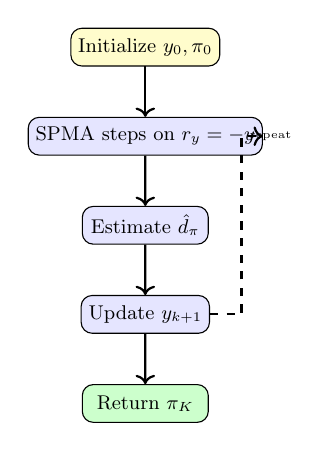
\begin{tikzpicture}[node distance=0.8cm, scale=0.8, transform shape,
        box/.style={draw, rounded corners, fill=blue!10, minimum width=2cm, minimum height=0.6cm, font=\small}]
        \node[box, fill=yellow!20] (init) {Initialize $y_0, \pi_0$};
        \node[box, below=of init] (policy) {SPMA steps on $r_y=-y$};
        \node[box, below=of policy] (estimate) {Estimate $\hat{d}_\pi$};
        \node[box, below=of estimate] (dual) {Update $y_{k+1}$};
        \node[box, below=of dual, fill=green!20] (output) {Return $\pi_K$};
        
        \draw[->, thick] (init) -- (policy);
        \draw[->, thick] (policy) -- (estimate);
        \draw[->, thick] (estimate) -- (dual);
        \draw[->, thick] (dual) -- (output);
        \draw[->, thick, dashed] (dual.east) -- ++(0.5,0) |- node[right, font=\tiny] {repeat} (policy.east);
      \end{tikzpicture}
    \end{center}
  \end{columns}

  \note{
    \textbf{Slide 22}
    \begin{itemize}
      \item Show the overall loop structure.
      \item Outer loop updates $y$, inner loop updates policy.
      \item Point to the diagram.
    \end{itemize}
  }
\end{frame}

%============================================================================
% SLIDE 23: SPMA Loss
%============================================================================
\begin{frame}{Policy Player: SPMA Actor Loss}
  \textbf{Standard Policy Gradient Loss:}
  \[
  \mathcal{L}_{\text{PG}} = -\mathbb{E}\left[\log\pi(a|s) \cdot A(s,a)\right]
  \]
  
  \textbf{SPMA adds a ``stay close'' regularizer:}
  \begin{block}{SPMA Actor Loss}
  \[
  \mathcal{L}_{\text{SPMA}} = \mathbb{E}\left[-\Delta\log\pi \cdot A + \frac{1}{\eta}\underbrace{\left(\exp(\Delta\log\pi)-1-\Delta\log\pi\right)}_{\text{KL-like regularizer}}\right]
  \]
  \end{block}
  
  \textbf{Notation:}
  \begin{itemize}
    \item $\Delta\log\pi = \log\pi_{\text{new}}(a|s) - \log\pi_{\text{old}}(a|s)$: change in log-probability
    \item $A(s,a)$: advantage function
    \item $\eta$: step size parameter (chosen via Armijo line search)
  \end{itemize}

  \note{
    \textbf{Slide 23}
    \begin{itemize}
      \item Explain SPMA loss as PG + regularizer.
      \item The regularizer prevents policy from changing too fast.
      \item Similar idea to TRPO/PPO but different form.
    \end{itemize}
  }
\end{frame}

%============================================================================
% SLIDE 24: Occupancy Estimation
%============================================================================
\begin{frame}{Occupancy Estimation: MC vs MLE}
  \begin{columns}
    \column{0.48\textwidth}
    \textbf{Monte Carlo (our default)}
    \begin{block}{Tabular Estimator}
    \small
    $\hat d_\pi(s,a) = \frac{1-\gamma}{N}\sum_{i=1}^{N}\sum_{t=0}^{T} \gamma^t \mathbf{1}\{s_t^{(i)}=s, a_t^{(i)}=a\}$
    \end{block}
    \begin{itemize}
      \item Simple: count discounted visits
      \item Variance grows with $|\mathcal{S}||\mathcal{A}|$
    \end{itemize}
    
    \column{0.48\textwidth}
    \textbf{MLE (Barakat et al., 2024)}
    \begin{block}{Log-Linear Model}
    \small
    $\lambda_\omega(s,a) \propto \exp(\omega^\top \phi(s,a))$
    \end{block}
    \begin{itemize}
      \item Fit $\omega$ by max-likelihood
      \item Error: $O(\sqrt{m/n})$
      \item Independent of $|S||A|$!
    \end{itemize}
  \end{columns}
  
  \vspace{0.4cm}
  \begin{center}
  \textbf{Sanity check:} $\sum_{s,a} \hat d_\pi(s,a) \approx 1$ verified in all our tests
  \end{center}

  \note{
    \textbf{Slide 24}
    \begin{itemize}
      \item Two estimation approaches side-by-side.
      \item MC is simple but high variance.
      \item MLE scales better to high dimensions.
    \end{itemize}
  }
\end{frame}

%============================================================================
% SLIDE 25: NPG-PD Implementation
%============================================================================
\begin{frame}{Baseline: NPG--PD Implementation}
  \textbf{Same Lagrangian as Dual--SPMA:}
  \[
  L(\pi,\lambda) = J_r(\pi) + \lambda(J_c(\pi)-\tau)
  \]
  
  \begin{columns}
    \column{0.48\textwidth}
    \textbf{Primal (policy):}
    \begin{itemize}
      \item Natural PG on shaped reward\\
            $r_\lambda = r - \lambda c$
      \item Diagonal Fisher approximation
      \item Same actor-critic as SPMA
    \end{itemize}
    
    \column{0.48\textwidth}
    \textbf{Dual (constraint):}
    \[
    \lambda_{k+1} = [\lambda_k + \beta(J_c - \tau)]_+
    \]
    \begin{itemize}
      \item One NPG step per iteration
      \item Evaluate $J_c$ via Monte Carlo
    \end{itemize}
  \end{columns}
  
  \vspace{0.3cm}
  \begin{center}
  \textbf{Fair comparison:} Same networks, same hyperparameters where possible
  \end{center}

  \note{
    \textbf{Slide 25}
    \begin{itemize}
      \item NPG-PD uses same Lagrangian, different policy update.
      \item We ensure fair comparison by using same architecture.
    \end{itemize}
  }
\end{frame}

%============================================================================
% SLIDE 26: CMDP Example
%============================================================================
\begin{frame}{Example: Constrained Safety CMDP}
  \textbf{Problem:} Maximize reward subject to safety constraint
  \[
  \max_\pi J_r(\pi) \quad \text{s.t.} \quad J_c(\pi) \le \tau
  \]
  where $J_r(\pi) = \mathbb{E}_\pi[\sum_t \gamma^t r(s_t,a_t)]$ and $J_c(\pi) = \mathbb{E}_\pi[\sum_t \gamma^t c(s_t,a_t)]$.
  
  \vspace{0.2cm}
  \textbf{Dual--SPMA approach:}
  \begin{enumerate}
    \item Build dual variable: $y_\lambda(s,a) = \lambda c(s,a) - r(s,a)$
    \item Policy sees shaped reward: $r_y = -y = r - \lambda c$
    \item Run SPMA inner loop on $r_y$
    \item Update dual: $\lambda_{k+1} = [\lambda_k + \beta(J_c(\pi_k) - \tau)]_+$
  \end{enumerate}
  
  \vspace{0.2cm}
  \begin{center}
  \fbox{\parbox{0.8\textwidth}{\centering
    \textbf{SPMA vs NPG--PD:} Same dual update, different policy optimizer!\\
    Only difference is Step 3: SPMA loss vs.\ natural gradient
  }}
  \end{center}

  \note{
    \textbf{Slide 26 --- End of Speaker 3's section}
    \begin{itemize}
      \item Show how CMDP fits our framework.
      \item SPMA and NPG-PD differ only in policy step.
      \item Transition to Speaker 4 for experiments.
    \end{itemize}
  }
\end{frame}

%============================================================================
\section{Experiments}
%============================================================================

%============================================================================
% SLIDE 27: Roadmap
%============================================================================
\begin{frame}{Roadmap}
  \begin{enumerate}
    \item[\cmark] Background: Reinforcement Learning
    \item[\cmark] Motivation: Convex MDPs
    \item[\cmark] Problem Formulation: Fenchel Duality
    \item[\cmark] Related Work: ``Reward Is Enough'' \& SPMA
    \item[\cmark] Our Method: Dual--SPMA
    \item[$\rightarrow$] \textbf{Experiments}
    \item[] Conclusion \& Future Work
  \end{enumerate}
  
  \note{
    \textbf{Slide 27 --- Speaker 4 (Danielle) starts}
    \begin{itemize}
      \item Quick roadmap reminder.
      \item Now presenting experimental results.
    \end{itemize}
  }
\end{frame}

%============================================================================
% SLIDE 28: Experimental Setup
%============================================================================
\begin{frame}{Experimental Setup}
  \begin{columns}
    \column{0.48\textwidth}
    \textbf{Environments:}
    \begin{itemize}
      \item FrozenLake 4$\times$4 (tabular)
      \item Deterministic transitions
      \item Unsafe states = holes (cost $c=1$)
    \end{itemize}
    
    \textbf{Methods Compared:}
    \begin{itemize}
      \item Dual--SPMA (ours)
      \item NPG--PD baseline
    \end{itemize}
    
    \column{0.48\textwidth}
    \textbf{Metrics:}
    \begin{itemize}
      \item $J_r(\pi)$: reward return
      \item $J_c(\pi)$: cost return
      \item $J_c - \tau$: constraint violation
      \item $\sum \hat d_\pi$: estimator sanity
    \end{itemize}
    
    \textbf{Hyperparameters:}
    \begin{itemize}
      \item Discount $\gamma = 0.99$
      \item Safety threshold $\tau = 0.1$
      \item 30 outer iterations
      \item 2048 steps/rollout
    \end{itemize}
  \end{columns}

  \note{
    \textbf{Slide 28}
    \begin{itemize}
      \item Describe the experimental setup.
      \item FrozenLake is simple but illustrative.
      \item Fair comparison with same hyperparameters.
    \end{itemize}
  }
\end{frame}

%============================================================================
% SLIDE 29: Entropy Results
%============================================================================
\begin{frame}{Results: Entropy-Regularized RL}
  \begin{columns}
    \column{0.48\textwidth}
      \begin{center}
        \figurePlaceholder{$L(\pi,y)$ vs iterations\\[0.3cm](Add plot here)}\\
        {\small Saddle value $L(\pi,y)$ vs iterations}
      \end{center}
    \column{0.48\textwidth}
      \begin{center}
        \figurePlaceholder{$\sum \hat{d}_\pi$ vs iterations\\[0.3cm](Add plot here)}\\
        {\small $\sum_{s,a} \hat d_\pi(s,a)$ vs iterations}
      \end{center}
  \end{columns}
  
  \vspace{0.3cm}
  \textbf{Observations:}
  \begin{itemize}
    \item Saddle value $L(\pi,y)$ converges smoothly
    \item Occupancy estimate stays near 1 (estimator is consistent)
  \end{itemize}

  \note{
    \textbf{Slide 29}
    \begin{itemize}
      \item Show entropy-regularized results.
      \item Convergence is smooth.
      \item Estimator sanity check passes.
    \end{itemize}
  }
\end{frame}

%============================================================================
% SLIDE 30: CMDP Results
%============================================================================
\begin{frame}{Results: Constrained Safety (Dual--SPMA)}
  \begin{columns}
    \column{0.48\textwidth}
      \begin{center}
        \figurePlaceholder{$J_r, J_c$ vs iterations\\[0.3cm](Add plot here)}\\
        {\small $J_r(\pi_k)$ and $J_c(\pi_k)$ vs iterations}
      \end{center}
    \column{0.48\textwidth}
      \begin{center}
        \figurePlaceholder{Constraint violation\\[0.3cm](Add plot here)}\\
        {\small Constraint violation $J_c - \tau$ and $\lambda_k$}
      \end{center}
  \end{columns}
  
  \vspace{0.3cm}
  \textbf{Observations:}
  \begin{itemize}
    \item $\lambda$ increases when constraint violated, decreases otherwise
    \item Constraint violation $\to 0$ as training progresses
  \end{itemize}

  \note{
    \textbf{Slide 30}
    \begin{itemize}
      \item Show CMDP results for Dual-SPMA.
      \item Dual variable $\lambda$ adapts correctly.
      \item Constraint is eventually satisfied.
    \end{itemize}
  }
\end{frame}

%============================================================================
% SLIDE 31: Comparison Results
%============================================================================
\begin{frame}{Results: Dual--SPMA vs NPG--PD}
  \begin{columns}
    \column{0.48\textwidth}
      \begin{center}
        \figurePlaceholder{$J_r$ comparison\\SPMA vs NPG-PD\\[0.2cm](Add plot here)}\\
        {\small $J_r(\pi_k)$ vs outer iterations}
      \end{center}
    \column{0.48\textwidth}
      \begin{center}
        \figurePlaceholder{Constraint violation\\comparison\\[0.2cm](Add plot here)}\\
        {\small Constraint violation vs iterations}
      \end{center}
  \end{columns}
  
  \vspace{0.3cm}
  \textbf{Takeaways:}
  \begin{itemize}
    \item Both methods eventually satisfy the constraint
    \item SPMA: larger, geometry-aware steps
    \item NPG--PD: smoother but requires careful step-size tuning
  \end{itemize}

  \note{
    \textbf{Slide 31}
    \begin{itemize}
      \item Compare SPMA vs NPG-PD directly.
      \item Both achieve constraint satisfaction.
      \item Different convergence behavior.
    \end{itemize}
  }
\end{frame}

%============================================================================
% SLIDE 32: Heatmaps
%============================================================================
\begin{frame}{Results: Occupancy Heatmaps}
  \begin{center}
    % Placeholder for comparison heatmaps
    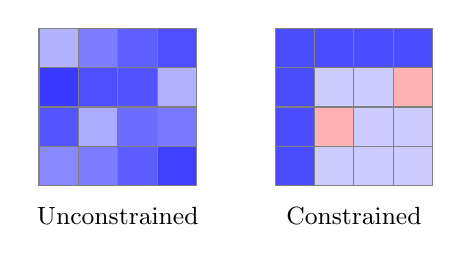
\begin{tikzpicture}[scale=0.5]
      % Left heatmap (Unconstrained)
      \foreach \x in {0,1,2,3} {
        \foreach \y in {0,1,2,3} {
          \pgfmathsetmacro{\intensity}{rnd*50+30}
          \fill[blue!\intensity] (\x,\y) rectangle (\x+1,\y+1);
        }
      }
      \draw[step=1,gray] (0,0) grid (4,4);
      \node[below] at (2,-0.3) {\small Unconstrained};
      
      % Right heatmap (Constrained) - with "safe path" pattern
      \begin{scope}[xshift=6cm]
        \foreach \x in {0,1,2,3} {
          \foreach \y in {0,1,2,3} {
            \pgfmathsetmacro{\safe}{(\x==0 || \y==3) ? 70 : 20}
            \fill[blue!\safe] (\x,\y) rectangle (\x+1,\y+1);
          }
        }
        \fill[red!30] (1,1) rectangle (2,2); % hole
        \fill[red!30] (3,2) rectangle (4,3); % hole
        \draw[step=1,gray] (0,0) grid (4,4);
        \node[below] at (2,-0.3) {\small Constrained};
      \end{scope}
    \end{tikzpicture}
  \end{center}
  
  \begin{columns}
    \column{0.48\textwidth}
    \centering
    \textbf{Left: Unconstrained}\\
    Policy explores more broadly
    
    \column{0.48\textwidth}
    \centering
    \textbf{Right: Safety-Constrained}\\
    Policy avoids unsafe states (holes)
  \end{columns}

  \note{
    \textbf{Slide 32}
    \begin{itemize}
      \item Visual comparison of occupancies.
      \item Constrained policy clearly avoids dangerous areas.
      \item This is the whole point of CMDPs!
    \end{itemize}
  }
\end{frame}

%============================================================================
\section{Conclusion \& Future Work}
%============================================================================

%============================================================================
% SLIDE 33: Takeaways
%============================================================================
\begin{frame}{Takeaways \& Limitations}
  \textbf{The Recipe:}
  \[
  \text{Convex MDP} \xrightarrow{\text{Fenchel}} \text{Saddle-Point Game} \xrightarrow{\text{SPMA}} \text{Shaped-Reward RL}
  \]
  
  \textbf{What we built:}
  \begin{itemize}
    \item Dual--SPMA loops for entropy-regularized RL and constrained safety
    \item NPG--PD baseline for fair comparison
    \item Three occupancy estimators (tabular MC, feature MC, MLE)
  \end{itemize}
  
  \textbf{Limitations:}
  \begin{itemize}
    \item Experiments only in low-dimensional (tabular) environments
    \item MLE estimator not yet stress-tested on large continuous tasks
    \item Hyperparameter sensitivity not fully characterized
  \end{itemize}

  \note{
    \textbf{Slide 33}
    \begin{itemize}
      \item Summarize the main recipe.
      \item Be honest about limitations.
      \item This sets up future work.
    \end{itemize}
  }
\end{frame}

%============================================================================
% SLIDE 34: Future Work
%============================================================================
\begin{frame}{Future Work}
  \begin{enumerate}
    \item \textbf{Scale up:}
      \begin{itemize}
        \item Test on larger CMDPs (continuous states/actions)
        \item MuJoCo safety tasks
      \end{itemize}
    
    \item \textbf{Better estimation:}
      \begin{itemize}
        \item Evaluate MLE estimator on high-dimensional tasks
        \item Compare variance of different estimators
      \end{itemize}
    
    \item \textbf{More objectives:}
      \begin{itemize}
        \item Risk-sensitive RL
        \item Imitation learning via convex MDP
      \end{itemize}
    
    \item \textbf{Theoretical analysis:}
      \begin{itemize}
        \item Convergence rates for Dual--SPMA
        \item Sample complexity comparison with NPG--PD
      \end{itemize}
  \end{enumerate}

  \note{
    \textbf{Slide 34}
    \begin{itemize}
      \item Concrete roadmap for future work.
      \item Shows we understand the bigger picture.
    \end{itemize}
  }
\end{frame}

%============================================================================
% SLIDE 35: Q&A
%============================================================================
\begin{frame}{Q\&A}
  \centering
  {\Huge Questions?}
  
  \vspace{1cm}
  \begin{tabular}{ll}
    \textbf{Pegah:} & Background \& Motivation \\
    \textbf{Danielle:} & Problem Formulation \& Fenchel Duality \\
    \textbf{Shervin:} & Related Work \& Our Method \\
    \textbf{Ahmed:} & Experiments \& Conclusion \\
  \end{tabular}

  \note{
    \textbf{Slide 35 --- Q\&A (5 minutes)}
    \begin{itemize}
      \item Invite questions.
      \item Direct questions to the appropriate speaker.
    \end{itemize}
  }
\end{frame}

%============================================================================
% SLIDE 36: References
%============================================================================
\begin{frame}{References}
  \small
  \begin{enumerate}
    \item \textbf{Zahavy, T., et al.} (2021). ``Reward is Enough for Convex MDPs.'' \textit{NeurIPS 2021}. arXiv:2108.06389
    
    \item \textbf{Asad, A., et al.} (2024). ``Fast Convergence of Softmax Policy Mirror Ascent.'' \textit{arXiv:2405.09781}
    
    \item \textbf{Ding, D., et al.} (2020). ``Natural Policy Gradient Primal-Dual Method for Constrained Markov Decision Processes.'' \textit{NeurIPS 2020}
    
    \item \textbf{Barakat, A., et al.} (2024). ``Reinforcement Learning with General Utilities: Simpler Variance Reduction and Large State-Action Space.'' \textit{ICML 2024}
    
    \item \textbf{Schulman, J., et al.} (2015). ``Trust Region Policy Optimization.'' \textit{ICML 2015}
    
    \item \textbf{Sutton, R. \& Barto, A.} (2018). ``Reinforcement Learning: An Introduction.'' \textit{MIT Press}
  \end{enumerate}

  \note{
    \textbf{Slide 36}
    \begin{itemize}
      \item List key references.
      \item Zahavy et al.\ is the main theoretical foundation.
      \item Asad et al.\ is the SPMA paper.
    \end{itemize}
  }
\end{frame}

%============================================================================
% BACKUP SLIDES
%============================================================================
\appendix

\begin{frame}{Backup: Flow Constraints (Occupancy Polytope)}
  \small
  The set $\mathcal{D}$ of valid occupancy measures satisfies \textbf{Bellman flow constraints}:
  
  For all states $s$:
  \[
  \sum_a d(s,a) = (1-\gamma)\rho(s) + \gamma\sum_{s',a'} P(s|s',a')\,d(s',a')
  \]
  
  Also: $d(s,a) \ge 0$ for all $(s,a)$
  
  \vspace{0.3cm}
  \textbf{Interpretation:}
  \begin{itemize}
    \item Flow into state $s$ = initial distribution + discounted flow from other states
    \item This is a \textbf{convex polytope} in $\mathbb{R}^{|S| \times |A|}$
  \end{itemize}
\end{frame}

\begin{frame}{Backup: Entropy-Regularized Conjugate}
  For entropy-regularized objective:
  \begin{align*}
  f(d) &= -\langle r,d\rangle + \alpha \sum_{s,a} d(s,a) \log d(s,a) \\[0.5em]
  f^\ast(y) &= \alpha \log\sum_{s,a} \exp\left(\frac{y(s,a)+r(s,a)}{\alpha}\right) \\[0.5em]
  \nabla f^\ast(y) &= \mathrm{softmax}\left(\frac{y+r}{\alpha}\right)
  \end{align*}
  
  The gradient is a softmax distribution---very convenient for computation!
\end{frame}

\begin{frame}{Backup: SPMA with Function Approximation}
  \small
  In function approximation, the SPMA projection step becomes:
  \[
  \theta_{t+1} = \arg\min_\theta \sum_s d^{\pi_t}(s)\; \mathrm{KL}\big(\pi_{t+1/2}(\cdot|s)\,\|\,\pi_\theta(\cdot|s)\big)
  \]
  
  This is a \textbf{convex optimization problem} (weighted KL minimization).
  
  \vspace{0.3cm}
  Equivalent to \textbf{softmax classification}:
  \begin{itemize}
    \item Labels: actions from $\pi_{t+1/2}$
    \item Weights: state occupancies $d^{\pi_t}(s)$
    \item Features: state representations
  \end{itemize}
\end{frame}

\begin{frame}{Backup: Algorithm Pseudocode}
  \footnotesize
  \textbf{Dual--SPMA Algorithm:}
  \begin{enumerate}
    \item Initialize dual variable $y_1 = 0$, policy $\pi_1$ randomly
    \item For $k = 1, 2, \ldots, K_{\text{outer}}$:
    \begin{enumerate}
      \item \textbf{Policy step:} Run $K_{\text{inner}}$ SPMA iterations on shaped reward $r_{y_k} = -y_k$
      \[
      \pi_{k+1} = \text{SPMA}(\pi_k, r_{y_k}, K_{\text{inner}})
      \]
      \item \textbf{Estimate occupancy:} Collect trajectories, compute $\hat{d}^{\pi_{k+1}}$
      \item \textbf{Dual step:} Update dual variable
      \[
      y_{k+1} = y_k + \alpha \left( \hat{d}^{\pi_{k+1}} - \nabla f^\ast(y_k) \right)
      \]
    \end{enumerate}
    \item Return final policy $\pi_K$
  \end{enumerate}
\end{frame}

\begin{frame}{Backup: Notation Summary}
  \small
  \begin{center}
  \begin{tabular}{cl}
    \toprule
    \textbf{Symbol} & \textbf{Meaning} \\
    \midrule
    $\mathcal{S}, \mathcal{A}$ & State and action spaces \\
    $\pi(a|s)$ & Policy (probability of action $a$ in state $s$) \\
    $r(s,a)$ & Reward function \\
    $c(s,a)$ & Cost function (for CMDPs) \\
    $\gamma$ & Discount factor \\
    $d_\pi(s,a)$ & Occupancy measure under policy $\pi$ \\
    $J(\pi)$ & Expected return \\
    $f(d)$ & Convex objective over occupancies \\
    $f^\ast(y)$ & Fenchel conjugate of $f$ \\
    $y$ & Dual variable \\
    $\lambda$ & Lagrange multiplier (for CMDPs) \\
    $\tau$ & Safety threshold \\
    $\eta$ & SPMA step size \\
    $\alpha$ & Dual step size \\
    \bottomrule
  \end{tabular}
  \end{center}
\end{frame}

\end{document}
